%&latex
\documentclass[10pt,a4paper]{article}
\usepackage[latin1]{inputenc}
\usepackage{amsmath}
\usepackage{amsfonts}
\usepackage{amssymb}
\usepackage{graphicx}
\usepackage{verbatim}
\usepackage{ulem}
\usepackage{wrapfig}
\usepackage{cite}
\usepackage[font=small,format=plain,labelfont=bf,up,textfont=it,up]{caption}
\usepackage[left=1.5cm,top=2cm,bottom = 2cm, right=2cm,nohead]{geometry}
\newcommand{\abs}[1]{\lvert#1\rvert}
\DeclareGraphicsExtensions{.pdf,.png,.jpg}
\begin{document}

\title{\bfseries \LARGE Fast Fourier Transforms: simulating Newtonian gravity for N bodies in one and two dimensions}
\author{Thomas W. Rogers}
\maketitle
\begin{abstract}
The FFT is applied in the simulation of Newtonian gravity in one and two dimensional space. It was found that systems could be modelled with reasonable accuracy for $ 0.45 < x/L<0.55$, with $N_g = 1024$. In this region the motion of point masses obey the analytic solution of the Poisson equation in one and two dimensions. It was found that the fundamental physics in the two dimensions was very different. More information is needed to determine whether the 2-D model could offer a good approximation of 3-D Newtonian Gravity.


\end{abstract}
\section{Introduction}
People have been fascinated by the motions of the celestial bodies since the dawn of mankind. The need for understanding the interactions between the sun, planets and stars has motivated people to seek a solution to the N-body problem. If the positions and velocities of a group of celestial bodies is known at one point in time, can one deduce the positions and velocities of the bodies at all other points in time? 

\begin{wrapfigure}{r}{0.3\textwidth}
\begin{center}
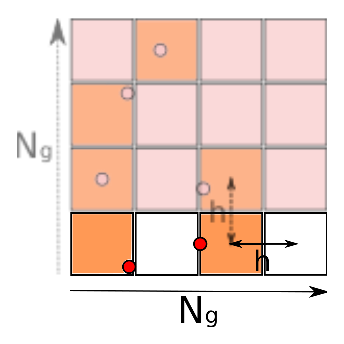
\includegraphics[width =0.3\textwidth]{grid.eps}
\caption{Demonstration of the unit grid, with the 2$^{nd}$ spatial dimension faded. Each point mass contributes all of it's mass to the closest element of the grid. The element spacing is $h=1/N_g$. In 2-D the area of each element is $h^2$}
\label{fig:Setup}
\end{center}
\end{wrapfigure}

Indeed the problem of finding the general solution to the $N$-body problem was found so challenging that in the late 1800s King Oscar II of Sweden established a prize for anyone that could find the solution. The prize was eventually awarded to Poincar\'{e}, although he did not even solve the original problem. However, he is renowned for providing the first mathematical description of chaotic behaviour in a dynamical system.

The problem is very difficult to solve analytically for $N \geq 3$ and therefore the numerical integration of the equation of motion for each body is the most practical approach. Considering Newton's law of universal gravitation for each particle in turn and then updating their positions and velocities by numerical integration is impractical for large $N$ as the scheme scales as $N(N-1)$.

In this investigation an alternative approach is considered in which the Poisson equation is solved in $n$ dimensions. The bodies are modelled as point masses distributed over a grid of size $N_g^n$. Each point mass contributes it's whole mass to the cell which it occupies. This is used to interpolate a density field that can be used in the solution of the gravitational Poisson equation,
\begin{equation}
\nabla\Phi(\textbf{x}) = k_n \rho(\textbf{x})\:,
\end{equation}
which relates the gravitational potential, $\Phi$, at position $\textbf{x}$ to the density field, $\rho$, at that position. $k_n$ is the scaling constant, i.e. $k_3=4\pi G$. This equation has a simple solution in the Fourier domain, so in our case of a discrete density field, it is convenient to use a discrete Fourier transform (DFT)\footnote{Throughout this investigation the \texttt{FFTW} subroutine library in \texttt{C} is used to perform FFT implementations of the DFTs.}. This reduces the problem to one that scales as $nN_g^n\log N_g$, which is a considerable improvement.

\section{Testing the \texttt{FFTW} subroutine library in 1-D}
The FFT plan creation functions in \texttt{FFTW} can be given a \texttt{FFTW\_MEASURE} or \texttt{FFTW\_ESTIMATE} flag. \texttt{FFTW\_MEASURE} tests the execution times of several different FFT algorithms. This is very useful for efficiency if the same plan is executed many times. The \texttt{fftw\_plan\_dft\_r2c\_1d} function takes an array of real input values of size $n$ and outputs an \texttt{fftw\_complex} array of size $n/2+1$ which is of C's native complex type. The output array describes the whole of the FFT of the real function through the reality condition,

\begin{equation}
\stackrel{{}_{\sim}\phantom{00|}}{\Phi_{-k}}=\stackrel{{}_{\sim}\phantom{00|}}{\Phi^{*}_{+k}}
\end{equation}

The implementation of the \texttt{FFTW} library was tested on some simple 1-D functions and compared against their analytic Fourier transforms.

\begin{figure}[h!]
\begin{center}
\includegraphics[width =0.3\textwidth, angle = -90]{sine.eps}
\includegraphics[width =0.3\textwidth, angle = -90]{sine_k.eps}
\caption{The imaginary component, \textbf{right}, of the FFT of $\sin{0.04\pi i}$, \textbf{left}, in grid units. From comparing the output with the analytic FFT, the discrete Fourier index $k$ maps to the continuous spatial frequency as $K=k/N_g$.}
\label{fig:tophat}
\end{center}
\end{figure}

\begin{figure}[h!]
\begin{center}
\includegraphics[width =0.3\textwidth, angle = -90]{tophat.eps}
\includegraphics[width =0.3\textwidth, angle = -90]{tophat_k.eps}
\caption{A top-hat, \textbf{left}, transforms to a sinc function, \textbf{right}. The sharp edge in the spatial domain causes ringing in the Fourier domain due to the Gibb's phenomenon.  }
\label{fig:tophat}
\end{center}
\end{figure}

\begin{figure}[h!]
\begin{center}
\includegraphics[width =0.3\textwidth, angle = -90]{guass.eps}
\includegraphics[width =0.3\textwidth, angle = -90]{guass_k.eps}
\caption{A Gaussian, \textbf{left}, transforms to a Gaussian function, \textbf{right}, with a different variance}
\label{fig:tophat}
\end{center}
\end{figure}

\newpage
\section{The use of FFT's in image manipulation}
The implementation of the \texttt{FFTW} 2-D forward and backward FFTs was tested on the face of Professor Blackett, former Head of the Physics Department at Imperial College. Observing the convolution theorem,
\begin{equation}
\mathcal{F}\{ f(x,y)*K(x,y)\}=\mathcal{F}\{ f(x,y)\}\times\mathcal{F}\{ K(x,y)\}\: ,
\end{equation}
one can convolve Blackett's face, $f(x,y)$, with a variety of different kernels, $K(x,y)$, by finding the product of Blackett's face and the kernel in the fourier domain. 

As the Fourier transform of a Guassian is another Guassian function, a Guassian kernel reduces high frequency components in the frequency domain. The result of such an operation is the blurring of an image as in  Fig.~\ref{fig:SimpleFilters}, left. If a uniform disk is used as the high pass filter instead, Fig.~\ref{fig:SimpleFilters}, left but one, the filtered image produces ringing effects along the intensity edges, which is due to the Gibb's phenomenon when transforming the sharp edges of the disk back into the spatial domain.

\begin{figure}[h!]
\begin{center}
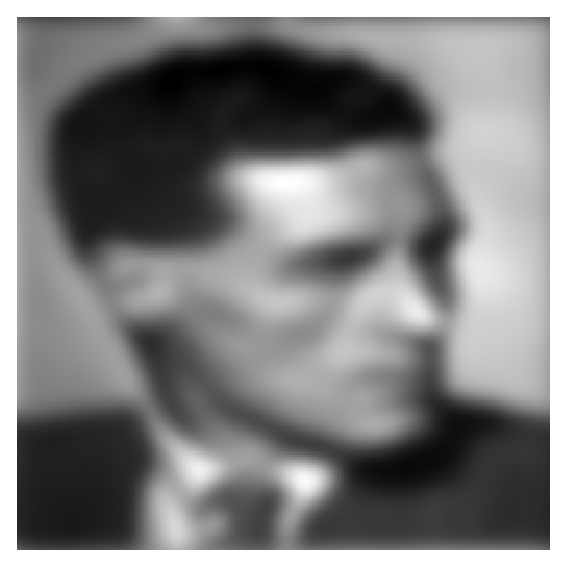
\includegraphics[width =0.2\textwidth]{BlackettGaussBlur.eps}
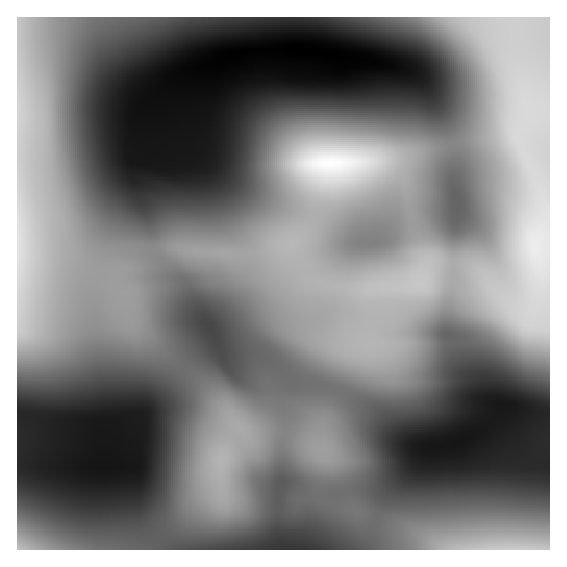
\includegraphics[width =0.2\textwidth]{BlackettHighPass.eps}
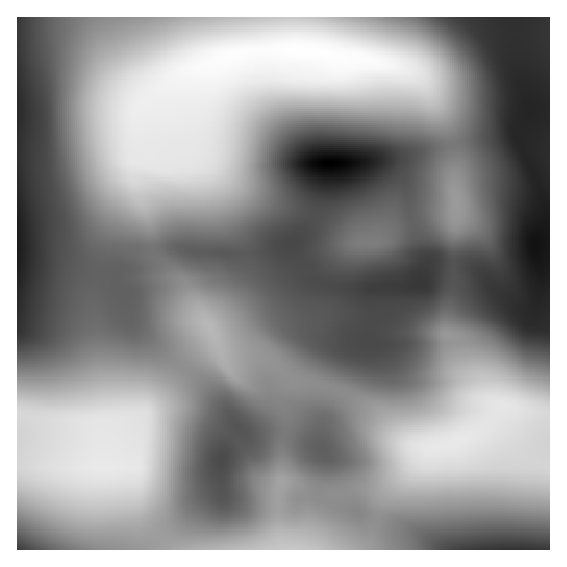
\includegraphics[width =0.2\textwidth]{BlackettLowPass.eps}
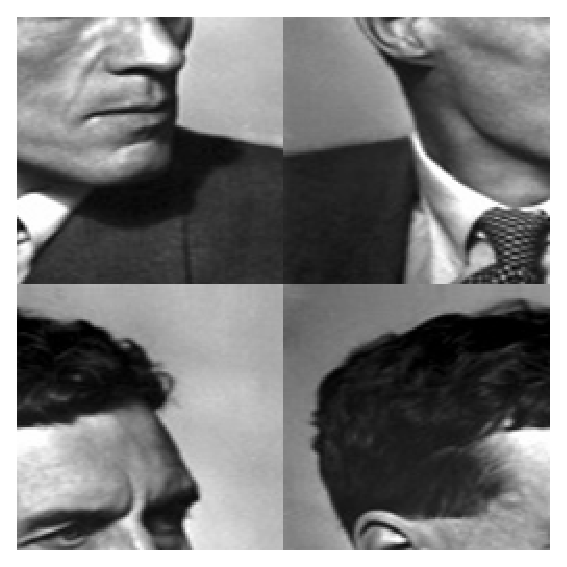
\includegraphics[width =0.2\textwidth]{BlackettSplitCenter.eps}
\caption{\textbf{Left: }The result of convolving Blackett's face with a Guassian. To get an isotropic smoothing the Guassian was centred in the kernel. However, this caused the image to be split about the centre so the image was recombined using a Dirac delta, right. \textbf{Centre: }High and low pass filters respectively. One can observe the ringing at the intensity edges due to the Gibb's phenomenon \textbf{Right: }A Dirac delta function at the centre of the kernel led to a four way splitting of the image. Shows the periodic properties of the FFT and how convolving with a Dirac function samples the image}
\label{fig:SimpleFilters}
\end{center}
\end{figure}

Taking the Laplacian of an image is an isotropic measure of the 2$^{nd}$ spatial derivative of the image. It therefore highlights regions of rapid intensity change and can be used in edge detection techniques.  However, the Laplacian kernel is sensitive to noise so it is important to smooth the image with a Guassian smoothing filter. Because the convolution operation is associative the combined effect is the same as convolving the image with the Laplacian of a Guassian, so the kernel becomes,
\begin{equation}
K(x,y) = -\frac{1}{\pi \sigma^{4}}\left[1-\frac{x^2+y^2}{2\sigma^2} \right]e^{-\frac{x^2+y^2}{2\sigma^2}}\: ,
\end{equation}
where $\sigma$ is the standard deviation of the Guassian. The result of such an operation is shown in Fig.~\ref{fig:EdgeDetection}.


\begin{figure}[h!]
\begin{center}
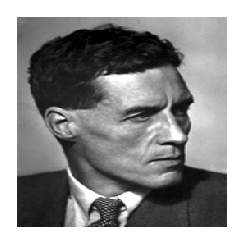
\includegraphics[width =0.3\textwidth]{Blackett.eps}
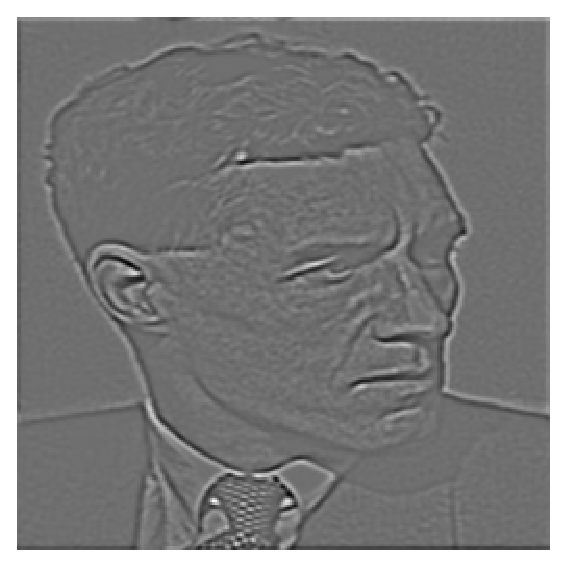
\includegraphics[width =0.3\textwidth]{BlackettEdgeDetection.eps}
\caption{\textbf{Left:} before and \textbf{Right:} after convolving Blackett's face with the Laplacian of a Guassian kernel. One can see that after the operation, regions of rapid intensity change, such as the boundary between his face and the background, are highlighted. Notice how the periodic nature of the DFT highlights the difference in intensity between the top and bottom of the image leading to the dark band.}
\label{fig:EdgeDetection}
\end{center}
\end{figure}

\section{Analytic solution for a point mass in $n$ dimensions}
The Newtonian potential is a solution of the n-D Poisson equation,
\begin{equation}
\nabla^2 \Phi(\textbf{x}) = f(\textbf{x})
\end{equation}
where $f$ is a compactly supported integrable function, at the position $\textbf{x}$. $\Phi$ is defined by the convolution\footnote{Another way of calculating the Newtonian potential would be to multiply $\Gamma$ by $\rho$ in the Fourier domain }, 
\begin{equation}
\Phi(\textbf{x}) = \Gamma * f(\textbf{x})\: ,
\end{equation}
where $\Gamma$, the Newtonian kernel, is defined by, 

\begin{equation}
  \Gamma(\textbf{x}) = \left\{ 
  \begin{array}{l l}
    \frac{1}{2}|\textbf{x}| & n=1\\
     \frac{1}{2\pi}ln|\textbf{x}| & n=2\\
    \frac{1}{n(2-n)\omega_n}|\textbf{x}|^{2-n} & d>2\\
  \end{array} \right.
\end{equation}
Here $\omega_n$ is the unit n-ball (i.e. the unit sphere in 3-D). 

Now consider the Poisson equation in 1-D,\footnote{For 3-D $k_3=4\pi G$, however for 1-D and 2-D $k_1$ and $k_2$ are unknown because we can not measure them in an inherently 3-D world. We shall take units of $k_1=k_2=1$}
\begin{equation}
\frac{d\Phi}{dx_1} = k_1\rho(x_1)
\end{equation}
If we choose a point of mass $M_1$ at $a$ such that, $\rho(x_1)=M_1\delta(x_1-a)$, then when we convolute we just shift the Newtonian kernel so,
\begin{equation}
\Phi(x_1)=\frac{k_1M_1}{2}|x_1-a|
\end{equation}
Doing the same in 2-D, with a mass, $M_2$, at $\textbf{b} = (b_1,b_2)$, we arrive at,
\begin{equation}
\Phi(\vec{x_2})=\frac{k_2M_2}{2\pi}ln|\textbf{x}_2-\textbf{b}|
\end{equation}
Finally, doing the equivalent in 3-D, with a mass, $M_3$, at $\textbf{c} = (c_1,c_2,c_3)$, and knowing $k_3=4\pi G$ we get,
\begin{equation}
\Phi(\textbf{x}_3)=-\frac{GM_3}{|\textbf{x}_3-\textbf{c}|}\:,
\end{equation}
which agrees with Newton's gravitational law as we would expect.

Now in each of these cases, if we had $N$ point masses, then the potential that one would expect is a superposition of the potential due to each. Also notice how for each case the potential is only radially dependent, which seems intuitive. One way of thinking about the change in potential is that when confined to less than 3-D all of the mass flux can only act in those dimensions which results in a different potential. In the 1-D case, all of the mass flux acts in one direction and there is no inverse square law, so one would expect a constant acceleration over the entirety of space. 

One must note that the constants of proportionality for 1-D and 2-D can not be determined, as we are existing in a 3-D world and it is inherently difficult to measure constants that exist in a 1-D world. However, by taking the constant into the mass units then one can test the the shape of the solutions.
 \newpage
\section{1-D Gravity}
Working in 1-D and discretising onto an array of size $N_g$ using the central approximation scheme, the Poisson equation becomes,
\begin{equation}
N_g^2\left(\Phi_{i+1}-2\Phi_{i}+\Phi_{i-1}\right) = \rho_i \:,
\end{equation}
where $i$ is the grid index. Now taking the DFT we get that,
\begin{equation}
\stackrel{{}_{\sim}\phantom{0}}{\Phi_k} = \frac{\stackrel{{}_{\sim}}{\rho_k}}{2N_g^2\left[cos\left(\frac{2\pi k}{N_g}\right)-1\right]}\:,
\end{equation}
where k is wave index. Hence, it is easy to solve for the potential in the Fourier domain.

Since gravity is a conservative force\footnote{This must be the case as in 1-D there is only one possible loop integral and by the fundamental theorem of calculus it is always zero} it satisfies the derivative condition,
\begin{equation}
a(x) = -\frac{d\Phi}{dx}\:,
\end{equation}
where $a$ is the acceleration. This acceleration can also be determined using a central approximation scheme,
\begin{equation}
a_i = -\frac{N_g}{2}\left(\Phi_{i+1}-\Phi_{i-1}\right) \:.
\end{equation}
Now it is possible to numerically integrate this acceleration and update the new positions and velocities of the particles in time. Note that it was important to observe the periodic boundary conditions of the FFT such that the potential was continuous through the boundaries. This would prevent infinite accelerations at the boundaries due to a discontinuity in the potential.

\subsection{\texttt{C++} implementation}

A \texttt{Gravity} class was written to keep track of the assignment of dynamic memory for the numerous arrays that were required in tracking the particle positions, masses, velocities, accelerations etc. In initialising the density field a particle of mass, $m/k_1$, would be put into the closest array index by rounding $x/h$ either up or down to the nearest integer. An \texttt{addParticle} function was created to make it easy to add particles with different initial conditions. In the object constructor an \texttt{ftw\_plan} was created with the \texttt{FFTW\_MEASURE} flag in order to find the most efficient algorithm for performing the FFTs in the time loop. Where possible an $N_g$ of a power of 2 was  used to further improve efficiency.

For the time evolution the positions and velocities (in real units) of each particle were updated with a timestep $dt$ via the Leapfrog method, which provides a global accuracy of $\mathcal{O}(dt^2)$ and is stable for periodic solutions so long as $dt < 1/\omega$, where $\omega$ is the frequency of oscillation\footnote{This fact was realised during the investigation - ``Dynamics of a double pendulum and stability of numerical methods on solving oscillatory problems"}. Then the real position of each particle was interpolated onto the grid and  the process was repeated. If a particle went off the grid (i.e. $x>L=1$ or $x<0$) then it's position was changed such that it looped round to the other side of the grid. This abides by the periodic nature of the whole model and ensures that masses are completely removed from the potential.
 
\subsection{Problems with periodic boundaries}
Using Eq. 9 we can validate out results against the analytic solution, Fig.~\ref{fig:SingleAnalytic}. One can see that it is important to consider scenarios where masses are close to the centre of the grid where the numerical solution is a better approximation of the analytic solution.

\begin{table}[h!]
\label{tab:ResultsUndamped}
\caption{Percentage difference between the analytic and numeric solutions at different $x$}
% title of Table
\centering
% used for centering table
\begin{tabular}{l c c c c c}
% centered columns (5 columns)
\hline\hline
Position, $x/L$ & 0.5 & 0.525 & 0.550 & 0.575 & 0.600 \\ [1ex]
Error, \% & 0 & 0.52 & 2.2 & 6.5 & 15 \\ [1ex]
\hline
\end{tabular}
\label{table:nonlin}
% is used to refer this table in the text
\end{table}
Table 1 shows how the boundary effect begins to take over for $x>5.5\, L$. For an accurate simulation of 1-D gravity it is therefore imperative to keep the particles within this range. It also implies that one would expect that only masses very close to the centre would obey the proper 1-D physics. 

Eq. 9 tells us that for two point masses in this region each should have an acceleration of magnitude $M_1/2$ and flips signs as the particles cross, Fig.~\ref{fig:velAccAnalytic}. In theory the particles would oscillate about the centre of mass with increasing amplitude, but in our model the gradient of the potential is effected by the periodic boundary conditions and the amplitude of oscillation stabilises.

\begin{figure}[h!]
\begin{center}
\includegraphics[width =0.5\textwidth, angle =-90]{singleAnalytic.eps}
\caption{A comparison of the of numeric and analytic solution shapes for the Poisson equation in the 1-D case with a point mass $m = 0.1\, kg/k_1$. One can see that close to the point mass the solutions match to a high degree of accuracy and the acceleration is constant as expected. However, as you get further from the point source the numeric solution converges at the boundaries, whereas the analytic solution diverges to infinity. This effect is an artefact of the periodic nature of the FFT. }
\label{fig:SingleAnalytic}
\end{center}
\end{figure}

\begin{figure}[h!]
\begin{center}
\includegraphics[width =0.3\textwidth, angle =-90]{accAnalytic.eps}
\includegraphics[width =0.3\textwidth, angle =-90]{velAnalytic.eps}
\caption{\textbf{Left: }The acceleration of $m_1$ as a function of time, $t$, in a high resolution grid, $N_g = 10000$, with two point masses, $m_1=m_2=0.01\, kg/k_1$, placed at $x_1=0.4999\,L$ and $x_2 = 0.5001\,L$. The systems start in the region where the potential matches the analytic solution. Therefore as expected there is a constant acceleration which changes direction as the particles cross. However, the acceleration becomes perturbed at larger times as the particles move into regions where the potential does not match the analytic solution. This acceleration leads to a velocity, \textbf{Left}, whose magnitude increases linearly in time and whose gradient changes sign as the particles cross.}
\label{fig:velAccAnalytic}
\end{center}
\end{figure}
The periodic boundary conditions also lead to an ``anti-gravity" effect whereby if the distance between two masses is $s > 0.5\, L$ then the shortest path between particles is through the periodic boundary and then the accelerations seem in the wrong direction,  Fig.~\ref{fig:boundaryEffect}. For $x_1 = 0.25\, L$ and  $x_2 = 0.75\, L$, one observes that the ``anti-gravity" and gravity forces are in equilibrium and the particles do not accelerate at all. 

\begin{figure}[h!]
\begin{center}
\includegraphics[width =0.325\textwidth, angle =-90]{edges.eps}
\includegraphics[width =0.325\textwidth, angle =-90]{Leap0.1.eps}
\caption{\textbf{Left: }The potential as a function of $x$ for two point masses, $m_1=m_2=0.01\, kg/k_1$, placed at $x_1=0.1\,L$ and $x_2 = 0.9\,L$. In the shortest distance between the two particles is through the periodic boundary. The periodicity of the model allows for particles to accelerate towards the boundaries as if the masses are repelled ``anti-gravity".  \textbf{Right: }Position as a function of time, $t$, for two point masses $m_1 = m_2 = 0.01\, kg/k_1$ start at $x_1 = 0.45 \,L$ and $x_2 = 0.55\,L$ with $dt=0.1\,s$. For this case, $dt < 1/\omega$ and so the Leapfrog is unstable as seen by the increasing amplitude until $375\, s$, where $|x_1-x_2| > 0.5$ and the ``anti-gravity" effect takes over until the masses pass through the grid boundary. This process will repeat with the centre of oscillation switching periodically}
\label{fig:boundaryEffect}
\end{center}
\end{figure}
\newpage
\newpage
\subsection{1-D potential for $N = 2$}
Fig.~\ref{fig:1DPotEqualMass} shows the potential for $N=2$ at two limiting cases,  $m_1 = m_2$ and $m_1>>m_2$. Again the potentials appear to follow the general shape of the analytic solution accept towards the boundaries.
\begin{figure}[h!]
\begin{center}
\includegraphics[width =0.3\textwidth, angle =-90]{equalMassPot.eps}
\includegraphics[width =0.3\textwidth, angle =-90]{diffMassPot.eps}
\caption{\textbf{Left: }The potential as a function of $x$ for two point masses, $m_1=m_2=0.01\, kg/k_1$, placed at $x_1=0.45\,L$ and $x_2 = 0.55\,L$. The potential is symmetric about the centre of the grid because the mass distribution is also symmetric about the centre of the grid \textbf{Right: }The potential as a function of $x$ for two point masses, $m_1=0.01\, kg/k_1$ and $m_2=0.001\, kg/k_1$, placed at $x_1=0.45\,L$ and $x_2 = 0.55\,L$. The small mass $m_2$ acts as a small perturbation to the uniform potential around the large mass $m_1$. Notice the continuity of the potential at the boundaries and that the average values of the potentials is zero due to the fact that the DC component was set to zero in the Fourier domain}
\label{fig:1DPotEqualMass}
\end{center}
\end{figure}
\newpage
\subsection{Varying grid size}
It was found that a grid size of $N_g = 1024$ gave a suitable degree of accuracy without costing too much in terms of processing time, Fig.~\ref{fig:phase}. However, one must consider whether a larger grid size is required for higher resolution when limiting the problem to the analytic region. 
\begin{figure}[h!]
\begin{center}
\includegraphics[width =0.325\textwidth, angle =-90]{phase.eps}
\includegraphics[width =0.325\textwidth, angle =-90]{accPhase.eps}
\caption{\textbf{Left: } Phase plot of $m_1$ for different $N_g$ when two point masses $m_1 = m_2 = 0.01\, kg/k_1$ start at $x_1 = 0.45 \,L$ and $x_2 = 0.55\,L$ with $dt=0.001\,s$. One can see that when the points cross the speed reaches a maximum. The width of the maximum increases with the inverse of the grid resolution, because the discontinuous acceleration acts over a larger distance. \textbf{Right: } Acceleration as a function of position x for $m_1$ under the same initial conditions. There is a discontinuity in the acceleration as the particles cross. A grid size of $N_g = 16$ results in a particularly large error in the acceleration at $x = 0.45\,L$. It is also apparent that in general $N_g = 1024$ is a suitable grid size.}
\label{fig:phase}
\end{center}
\end{figure}

\section{2-D Gravity}
Working in 2-D with units of $k_2=1$ and discretising onto a grid of size $N_g\times  N_g$ using the central approximation scheme, the Poisson equation becomes,
\begin{equation}
N_g^2\left(\Phi_{i+1,j}+\Phi_{i,j+1}-4\Phi_{i,j}+\Phi_{i-1,j}+\Phi_{i,j-1} \right) = \rho_{i,j} \:,
\end{equation}
where $i$ and $j$ are the grid indices. Now taking the DFT we get that,
\begin{equation}
\stackrel{{}_{\sim}\phantom{000|0}}{\Phi_{k_i,k_j}} = \frac{\stackrel{{}_{\sim}\phantom{0000}}{\rho_{k_i,k_j}}}{2N_g^2\left[cos\left(\frac{2\pi k_i}{N_g}\right)+cos\left(\frac{2\pi k_j}{N_g}\right)-2\right]}\:,
\end{equation}
where $k_i$ and $k_j$ are the wave indices for $i$ and $j$ respectively. And so for 2-D it is also easy to solve for the potential in the Fourier domain.

The acceleration now acts in 2-D so,
\begin{equation}
\textbf{a}(\textbf{x}) = -\nabla \Phi(\textbf{x})\:,
\end{equation}
where $\textbf{a}$ is the acceleration vector and $\textbf{x}$ is the position vector. This time in the discrete case  the two acceleration components can be found using a central approximation scheme,
\begin{equation}
a_i = -\frac{N_g}{2}\left(\Phi_{i+1,j}-\Phi_{i-1,j}\right) \:,
\end{equation}
\begin{equation}
a_j = -\frac{N_g}{2}\left(\Phi_{i,j+1}-\Phi_{i,j-1}\right) \:.
\end{equation}
Now the acceleration components can be numerically integrated in order to update the new components of position and velocity of the particles in time. Note again that it was important to observe the periodic boundary conditions of the FFT. The 2-D problem was implemented in much the same way in the class \texttt{Gravity\_2D}.
\newpage
\subsection{Two particles moving in 1-D inside 2-D space}
For two particles of equal mass that are initialised with zero velocity and zero separation in one dimension then the acceleration can be studied to check whether it fits the analytic solution, Fig.~\ref{fig:1Din2D}. The addition of an extra dimension radically changes the physics of the system. The analytic solution for the potential predicts that the acceleration should be radial and fall of as $1/r$, this agrees well with the numerical solution.

Also there is now a singularity in the velocity at the point at which the particles cross. This causes the position calculation to become unstable. As such for 2-D models collisions should be avoided to retain stability. By assigning an initial velocity it is very unlikely that particles will cross.

\begin{figure}[h!]
\begin{center}
\includegraphics[width =0.3\textwidth, angle =-90]{accPhase2d.eps}
\includegraphics[width =0.3\textwidth, angle =-90]{vel2D.eps}
\caption{\textbf{Left: }Acceleration of $m_1$ as a function of position $y_1$ , $t$, for 2 point masses $m_1 = m_2 = 0.01\, kg/k_2$ starting at $x_1 = x_2 =0.5 \,L$, $y_2= 0.55\,L$ and $y_2=0.45\,L$ with $dt=0.001\,s$ in a grid $N_g\times N_g = 1024\times 1024$. The acceleration is proportional to $1/y_1$ and hence agrees with the analytic solution for the potential. \textbf{Right: }The velocity as a function of time for the same case. The velocity of the particles along a 1-D line in 2-D space is fundamentally different to that in a purely 1-D space.}
\label{fig:1Din2D}
\end{center}
\end{figure}
\newpage
\subsection{Orbiting masses in 2-D}
Using Eq. 9 one can derive the initial conditions required for a two point masses to orbit each other. From Eq. 9 and working in units of $k_2=1$ we get the magnitude of the force acting on a point mass, $m$, a distance $r$ from a mass $M_2$,
\begin{equation}
|\vec{F}(r)| = m\frac{d\Phi}{dr} = \frac{mM_2}{2\pi r}
\end{equation}
For a stable orbit then this must equal the centripetal force, i.e.
\begin{equation}
\frac{mM_2}{2\pi r} = \frac{mv^2}{r}
\end{equation}
where $v$ is the tangential component of $m$'s speed. This gives,
\begin{equation}
v = \sqrt{\frac{M_2}{2\pi}}\:.
\end{equation}
This is very interesting as it predicts that regardless of the separation of the two masses in 2-D, as long as the tangential velocity satisfies Eq. 23 particle $m$ will be in stable orbit around $M_2$. This is shown in Fig.~\ref{fig:stableOrbits} using $M_2=0.1\, kg/k_1$, which gives a required $v\approx0.1262\,L/s$. As in the 1-D case the result breaks down at larger separations due to the periodic effect of the FFT.

\begin{figure}[h!]
\begin{center}
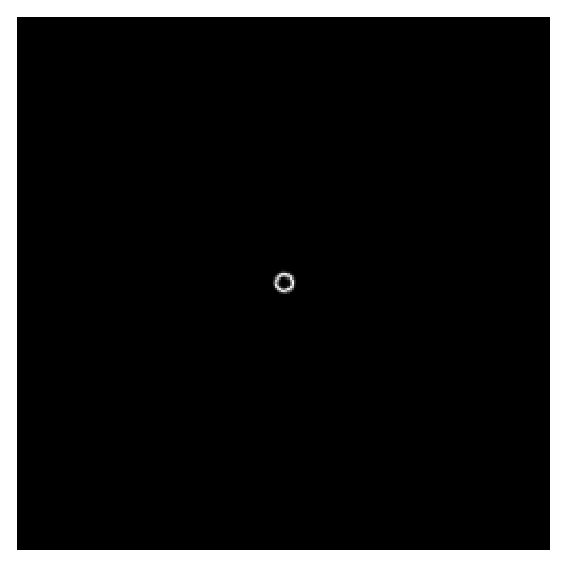
\includegraphics[width =0.2\textwidth]{traceOrbit0.01.eps}
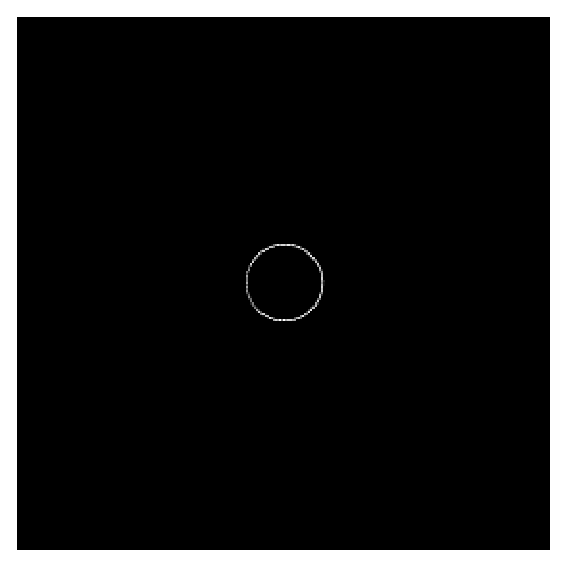
\includegraphics[width =0.2\textwidth]{traceOrbit0.05.eps}
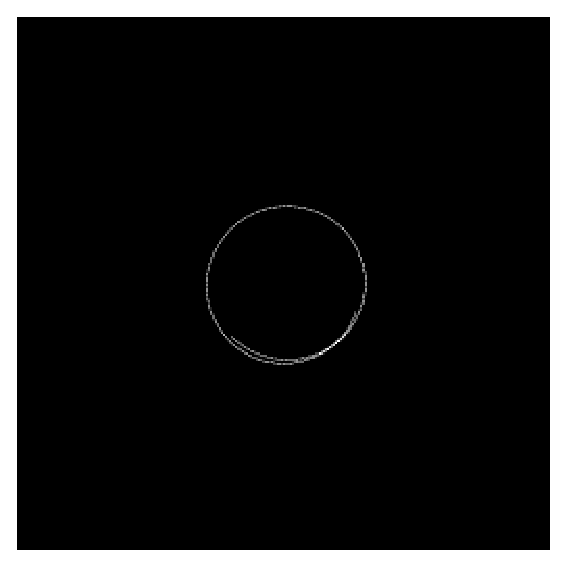
\includegraphics[width =0.2\textwidth]{traceOrbit0.1.eps}
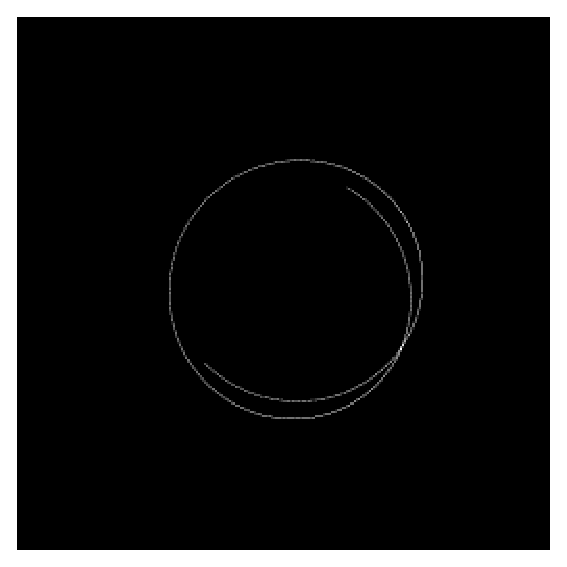
\includegraphics[width =0.2\textwidth]{traceOrbit0.15.eps}
\caption{Trajectory of orbtiting particle for different radial separations between the two point masses with $M_2=0.1\, kg/k_2$ at the centre. As expected from Eq.23, for any radial separation, as long as $v \approx 0.1262\,L/s$ $m$ will be in stable orbit around $M_2$. However as the separation gets large the computational solution no longer matches the analytic solution due to the periodic boundary effects and the orbits become unstable}
\label{fig:stableOrbits}
\end{center}
\end{figure}

Reducing $M_2$ and giving $m$ a push in only the x direction leads to a precessing elliptical orbit, because the position of the centre of rotation changes with time. Adding a third particle adds complexity to the system and chaos results as first suggested by Poincar\'{e}, Fig.~\ref{fig:unstableOrbits}.

\begin{figure}[h!]
\begin{center}
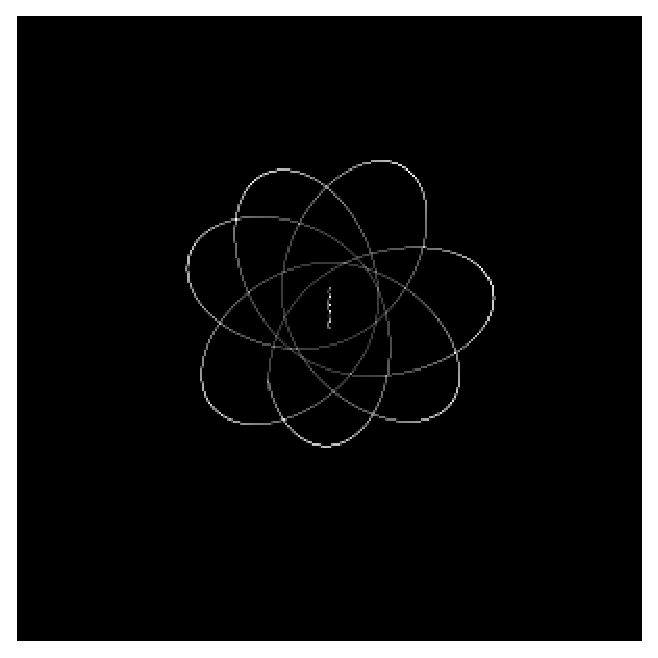
\includegraphics[width =0.3\textwidth]{orbit.eps}
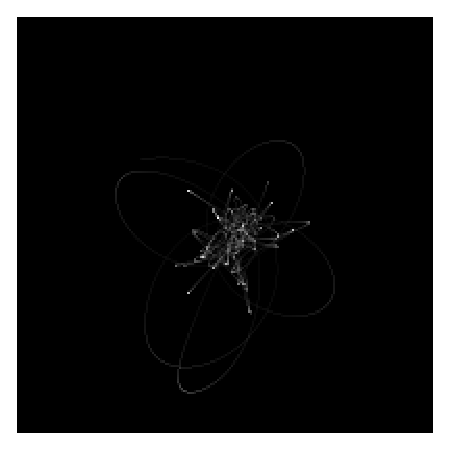
\includegraphics[width =0.3\textwidth]{2Nptrace.eps}
\caption{\textbf{Left: }The precession of the elliptic orbit of a small mass, $m_1$, around a heavy mass, $m_2$, at the origin. The orbit precesses because $m_2$ is only 10 times greater than $m_1$ and the force acting on it is enough to displace it from the centre and alter the centre of rotation. \textbf{Right: }The introduction of a 3$^{rd}$ point mass with random initial conditions. The introduction of the 3rd particle increases the complexity of the system and it appears chaotic. }
\label{fig:unstableOrbits}
\end{center}
\end{figure}

%\begin{figure}[h!]
%\begin{center}
%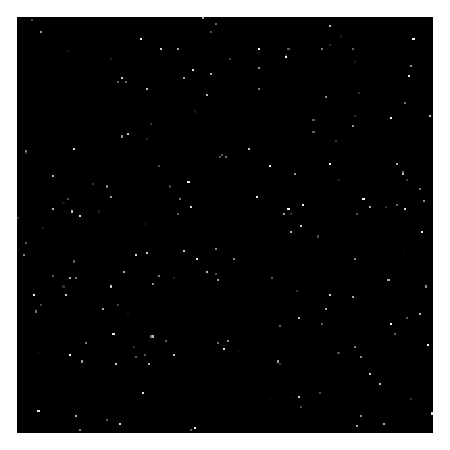
\includegraphics[width =0.3\textwidth]{Random199NpDen.eps}
%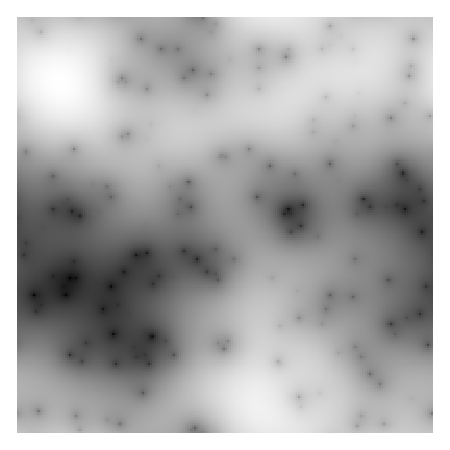
\includegraphics[width =0.3\textwidth]{Random199NpPot.eps}
%\caption{}
%\label{fig:1992D}
%\end{center}
%\end{figure}

%\begin{figure}[h!]
%\begin{center}
%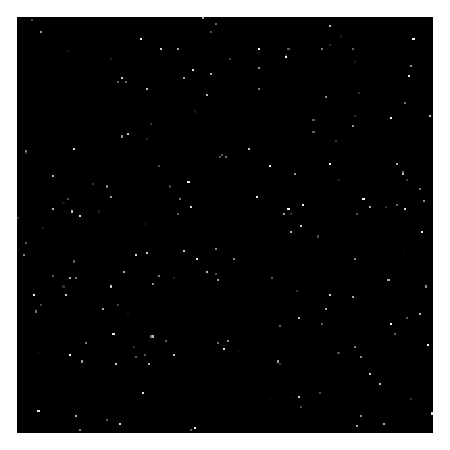
\includegraphics[width =0.3\textwidth]{Random199NpDen.eps}
%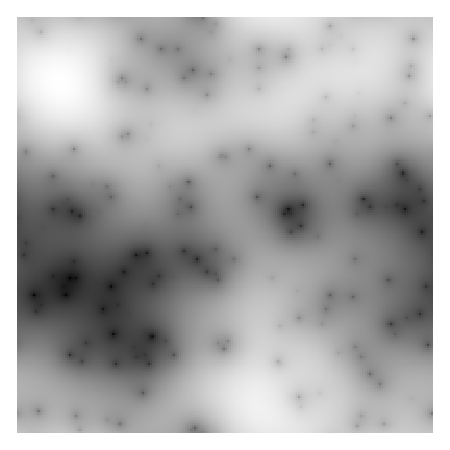
\includegraphics[width =0.3\textwidth]{Random199NpPot.eps}
%\caption{}
%\label{fig:1992D}
%\end{center}
%\end{figure}
%\begin{figure}[h!]
%\begin{center}

%\includegraphics[width =0.6\textwidth, angle=-90]{Random199Np.eps}
%\caption{}
%\label{fig:1992D3D}
%\end{center}
%\end{figure}
\newpage
\section{Conclusion}
The current method offers a good description of the Newtonian physics of one and two dimensional worlds, although it is questionable whether the assumption of a one and two dimensional Poisson equation are valid. The Poisson equation in 3-D is derived from Newton's Law of universal gravitation, which was found experimentally so it is hard to say whether such an equation holds in one and two dimensions. There is a clear difference between the solution of the N-body gravity in a space that is strictly one dimensional and confining motion to 1-D inside a 2-D space. As such it would be important to carry out further work in testing whether solving the Poisson equation in 2-D offers a good approximation to motion in a plane in 3-D. 

Working with $k_2=k_3=1$ and taking the ratios of the theoretical accelerations of a test mass a position $r$ from a test mass $M$ in 2 and 3-D,
\begin{equation}
\frac{|\textbf{a}_2|}{|\textbf{a}_3|} = \frac{\frac{M}{2\pi r}}{\frac{M}{4\pi r^2}} = 2r,
\end{equation}
suggests that the 2-D mathematics should provide a perfect representation of 3-D gravity at $r=1/2\, L$. However, this is at the boundary of the grid! So we have a problem where we have to put particles very close to the centre of the grid to avoid the boundary effects, yet this means that the model is largely underestimating accelerations for a 2-D plane inside 3-D.

Another problem is that when particles get close, the acceleration calculation becomes inaccurate due to the resolution of the potential. To resolve this problem, the program could be adapted so that is the particles are within a certain distance of each other, their potential is calculated using a direct some. Additionally there is not a simple way of modelling collisions accurately and efficiently. However, in two and three dimensions it is very unlikely that a collision will occur, so long as the point masses are initialised with a non-zero velocity.

A final point is that the method for numerical integration is sometimes inefficient when a point mass is moving with a relatively constant acceleration for a long period of time. In such a case it is unnecessary to carry out all of the individual time steps. To improve the efficiency and adaptive step algorithm could be used, which calculates the step size from an estimate of the local truncation error.

\begin{figure}[h!]
\begin{center}
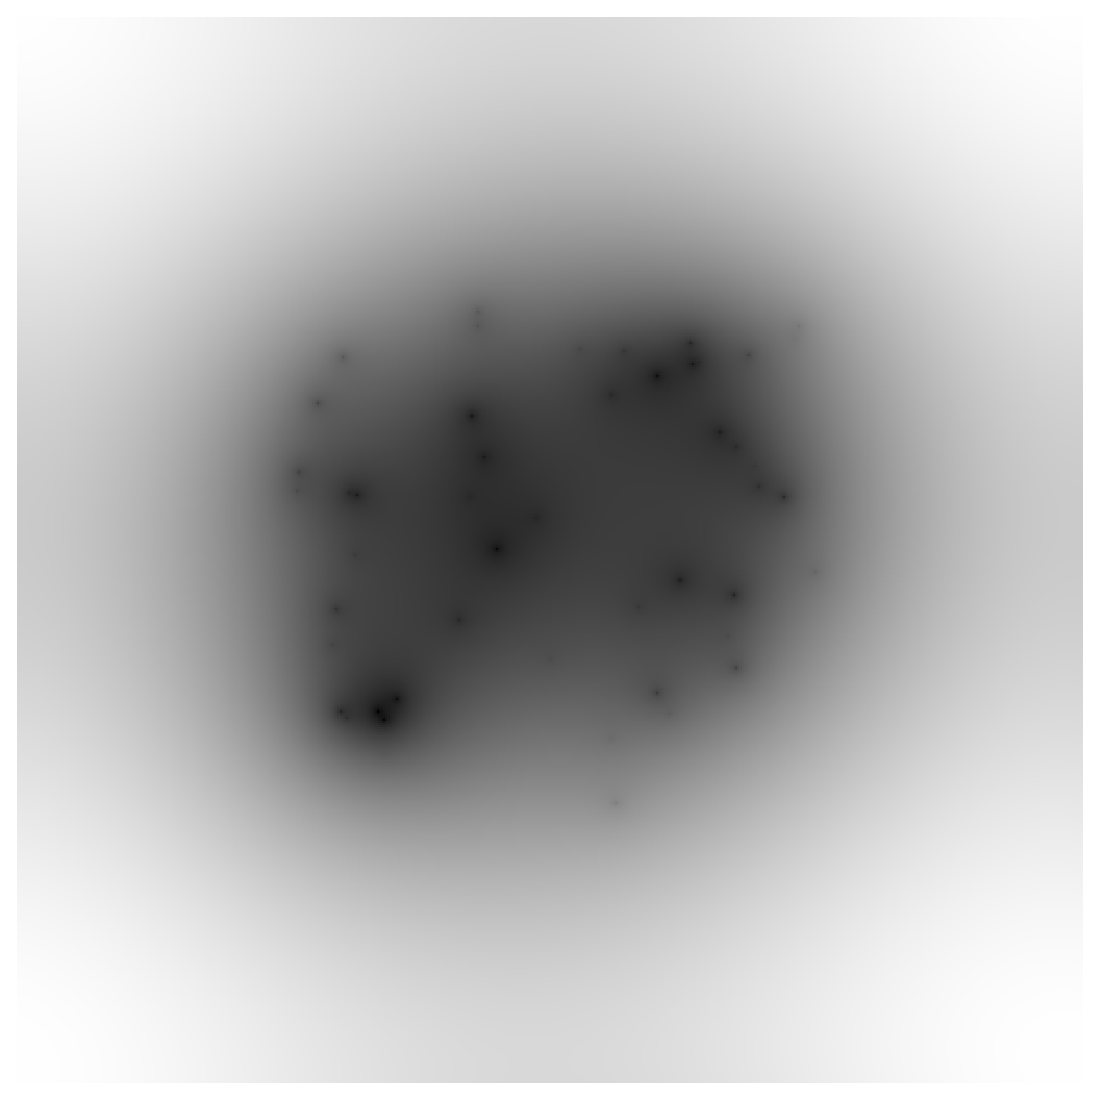
\includegraphics[width =0.2\textwidth]{t_0.4.eps}
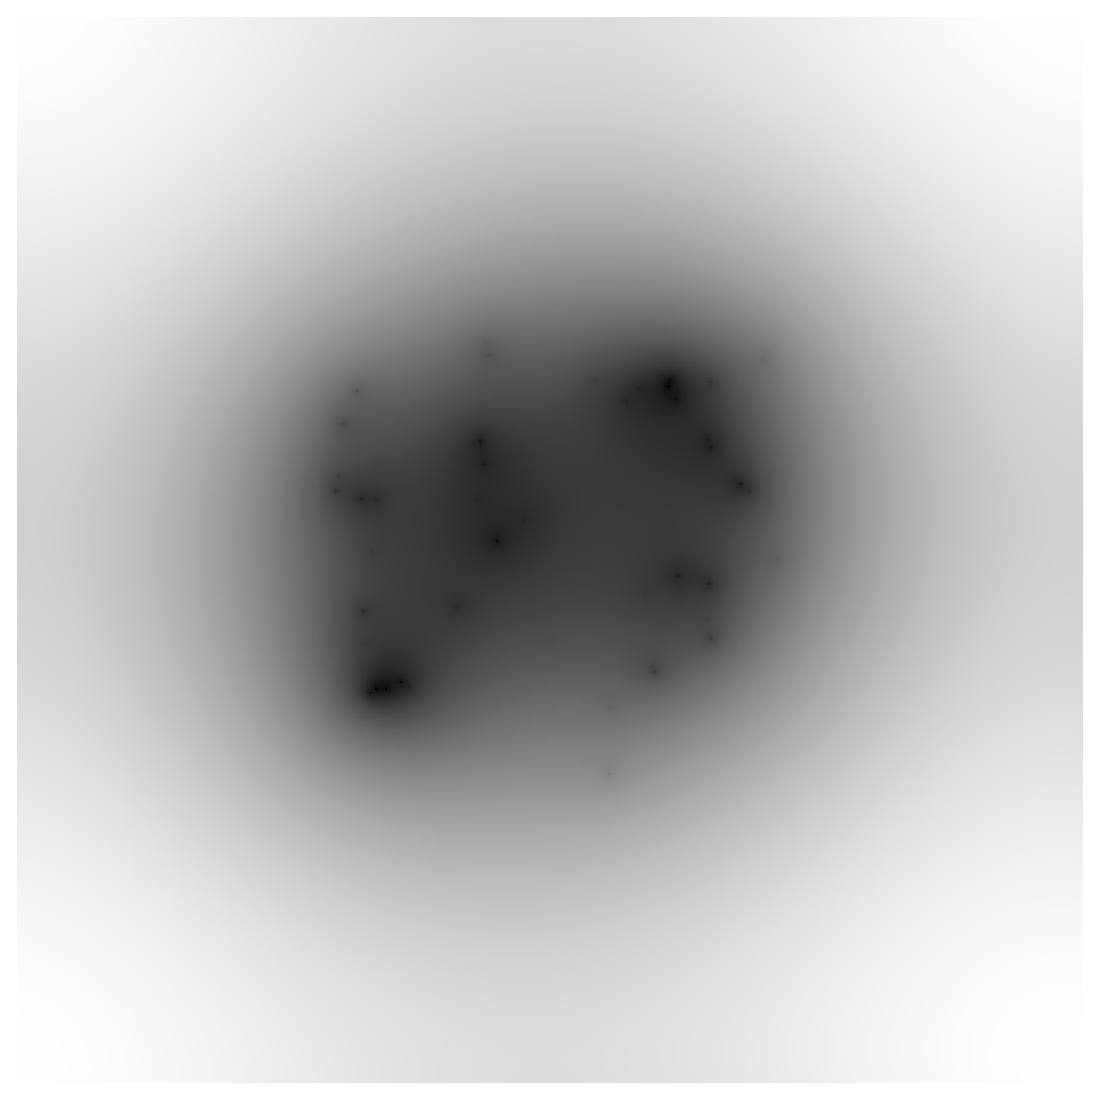
\includegraphics[width =0.2\textwidth]{t_8.6.eps}
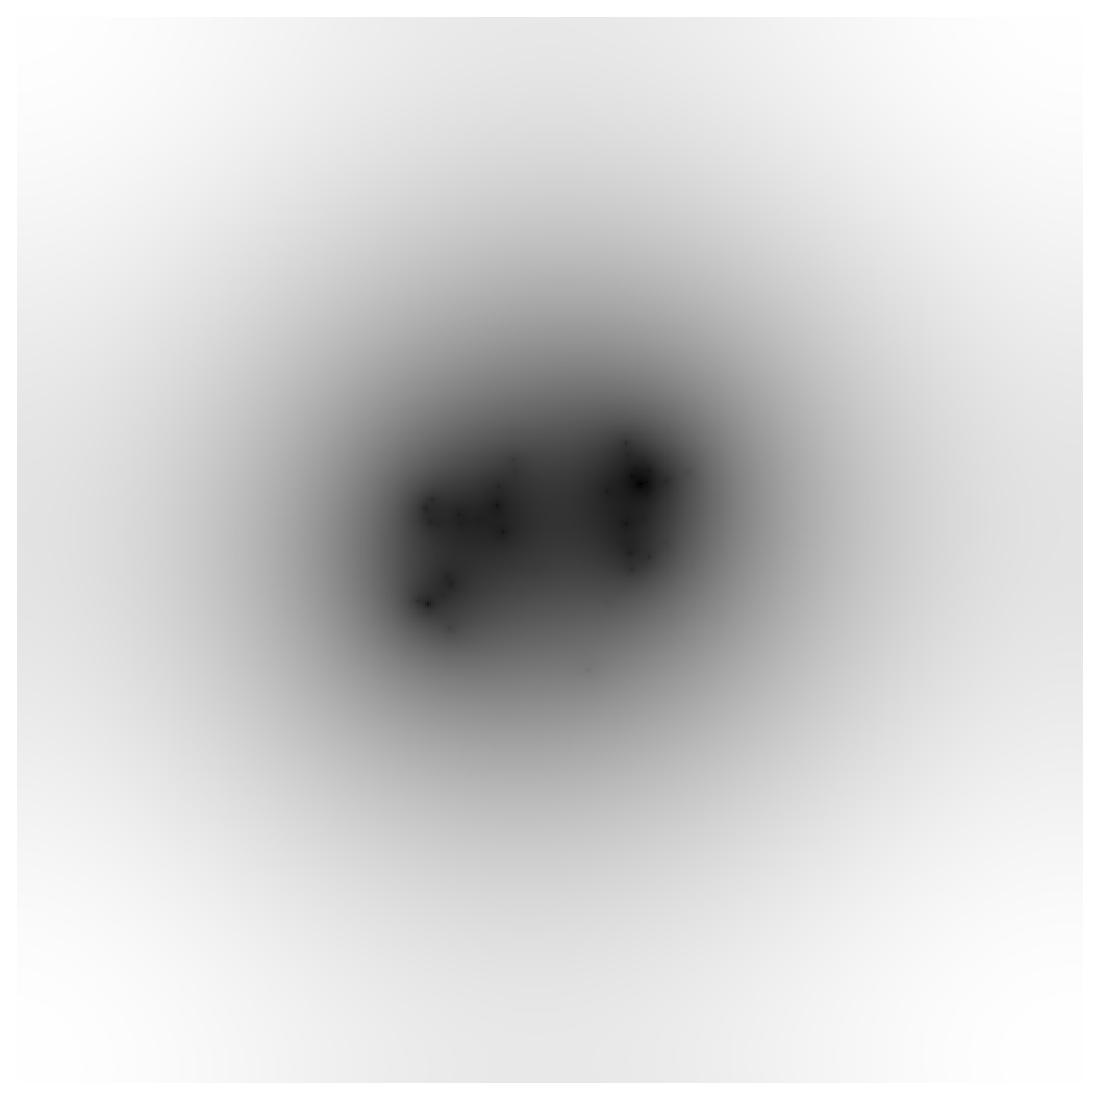
\includegraphics[width =0.2\textwidth]{t_17.4.eps}
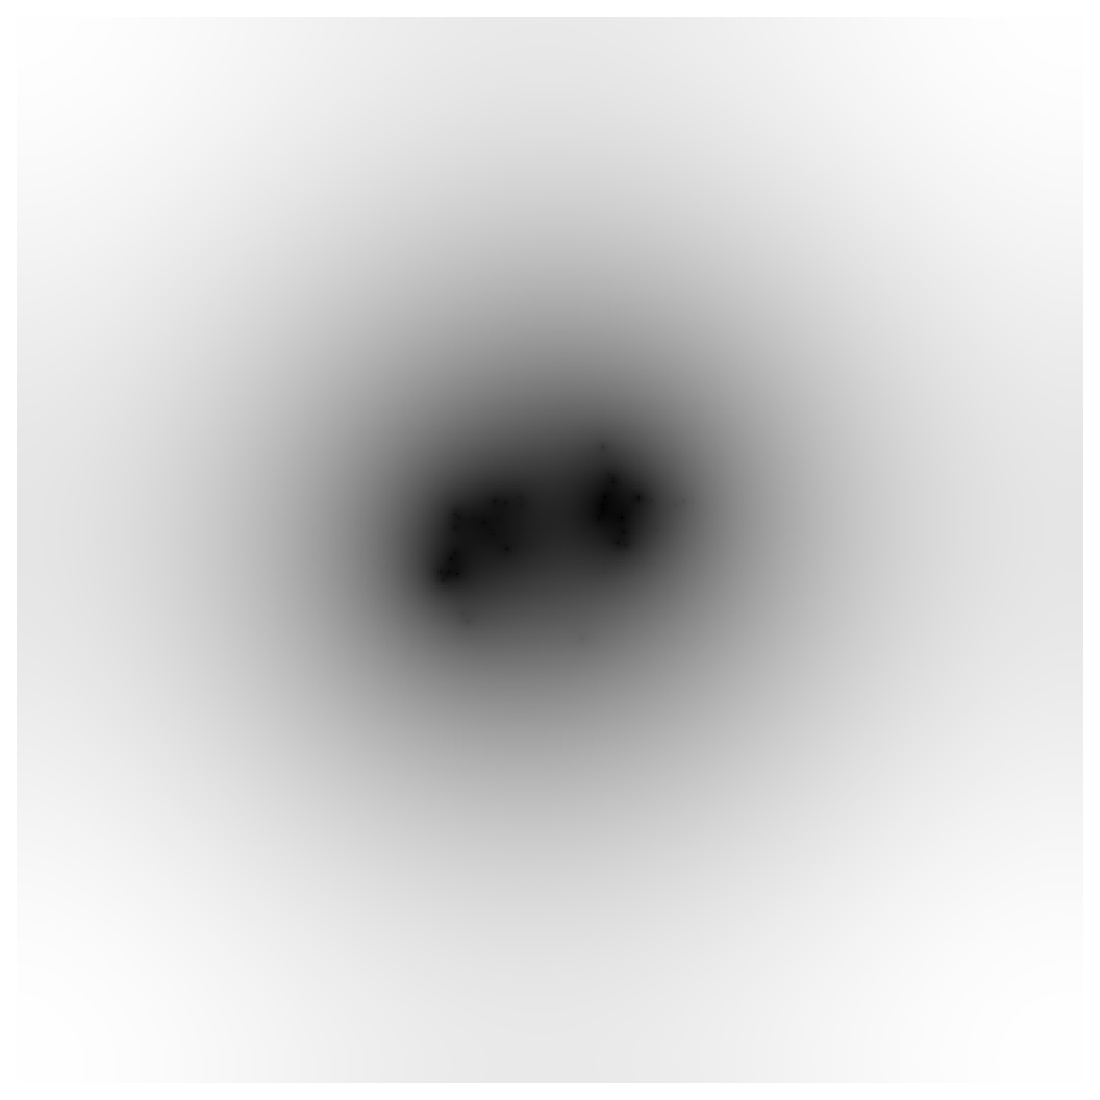
\includegraphics[width =0.2\textwidth]{t_19.eps}
\caption{Time evolution \textbf{left-right} of 50 point masses with randomly assigned initial conditions and restricted to the middle quarter of the grid. The masses gravitate towards the centre of mass and suggests that this computational model could possibly be extended to study the formation of stars in the interstellar medium}
\label{fig:1992D3D}
\end{center}
\end{figure}

$\approx$ 2458 Words- excluding captions and equations

\section{References}
\text{[1] \textbf{Diacu, F.}, \textit{`The solution of the n-body Problem"}, The Mathematical Intelligencer, 1996.}\\
\\
\text{[2] \textbf{Barrow-Green, J.}, \textit{``Oscar II's prize competition and the error in Poincar\'{e}'s memoir on the three body problem"}}\\
\\
\text{[3] \textbf{Contaldi, C.}, \textit{``Computational Physics Lecture Notes"}, Imperial College London, 2010.}\\
\\
\text{[4] \textbf{Contaldi, C.}, \textit{``Project B5: Simulation of Newtonian Gravity
"}, Imperial College London, 2010.}\\
\\
\text{[5] \textbf{Hunter, J.}, Ch. 2 of \textit{``Notes on Partial Diffferential Equations"}, University of California at Davis, 2010}\\
\\
\text{[6] \textbf{Evans, L.C}, Ch. 2 of \textit{``Partial Differential Equations"}, Providence: American Mathematical Society, 1998}

\end{document}
